% =============================================================================
%  ANNEXES
% =============================================================================
\cleardoublepage
\entete{Annexes}
% La page-titre « ANNEXES » isolée a été supprimée : l'entrée reste dans la
% table des matières, mais la première annexe commence directement.
\addcontentsline{toc}{chapter}{ANNEXES}

% Les tableaux et figures des annexes sont numérotés A.1, A.2, etc. :
% sans cela ils poursuivraient la numérotation du chapitre 4 et un renvoi
% du corps du texte deviendrait illisible.
\setcounter{table}{0}
\renewcommand{\thetable}{A.\arabic{table}}
\setcounter{figure}{0}
\renewcommand{\thefigure}{A.\arabic{figure}}

\chapter*{Annexe 1 : Guide d'entretien semi-directif}
\label{ann:guide}
\addcontentsline{toc}{chapter}{Annexe 1 : Guide d'entretien semi-directif}

\textbf{Destinataires :} personnel de la Fondation Jean Félicien Gacha et du
\emph{Think Tank} Fou'ndjem.\\
\textbf{Durée prévue :} 40 à 60 minutes.\\
\textbf{Période :} du 27 juin au 3 juillet 2026.

L'entretien s'ouvre sur la présentation de l'enquêteur et de l'objet de
l'étude, le rappel du caractère anonyme du traitement, la demande
d'autorisation d'enregistrement et le rappel de la liberté de ne pas répondre.

\subsection*{Thème 1 : Pratiques actuelles de valorisation}

\begin{enumerate}
  \item Comment un visiteur découvre-t-il aujourd'hui la Fondation et ses
        espaces ?
  \item De quelle manière les collections sont-elles inventoriées et
        documentées ?
  \item Quels supports utilisez-vous pour présenter les œuvres au public ?
  \item Quelle est la place du guide dans la visite ?
\end{enumerate}

\subsection*{Thème 2 : Difficultés rencontrées}

\begin{enumerate}\setcounter{enumi}{4}
  \item Quelles difficultés rencontrez-vous dans la gestion des collections ?
  \item Quels publics vous semblent aujourd'hui exclus de la découverte de la
        Fondation ? Pour quelles raisons ?
  \item Vous arrive-t-il de ne pas pouvoir répondre à une question de visiteur ?
        Dans quels cas ?
  \item Que devient l'information sur un visiteur une fois qu'il est reparti ?
\end{enumerate}

\subsection*{Thème 3 : Attentes vis-à-vis d'un dispositif à distance}

\begin{enumerate}\setcounter{enumi}{8}
  \item Que devrait permettre, selon vous, une visite à distance pour être
        satisfaisante ?
  \item Quelles informations sur une œuvre vous semblent indispensables ?
  \item Quelles craintes un dispositif automatique vous inspire-t-il ?
  \item Existe-t-il, à votre connaissance, des œuvres comparables aux vôtres
        conservées ailleurs ? Comment le savez-vous ?
\end{enumerate}

\subsection*{Thème 4 : Contraintes de moyens et pérennité}

\begin{enumerate}\setcounter{enumi}{12}
  \item Quels moyens humains pourraient être consacrés à l'entretien d'un tel
        dispositif ?
  \item Quel niveau de dépense annuelle vous semblerait soutenable ?
  \item Qui, au sein de la Fondation, pourrait en assurer l'administration
        courante ?
\end{enumerate}

L'entretien se clôt sur une question ouverte, « y a-t-il un point que nous
n'avons pas abordé et qui vous paraît important ? », puis sur les
remerciements.

% -----------------------------------------------------------------------------
\cleardoublepage
\chapter*{Annexe 2 : Questionnaire adressé aux visiteurs}
\label{ann:questionnaire}
\addcontentsline{toc}{chapter}{Annexe 2 : Questionnaire adressé aux visiteurs}

\textbf{Destinataires :} visiteurs présents sur le site, âgés de 18 ans et plus.
\textbf{Effectif recueilli :} 42 répondants. \textbf{Période :} juillet 2026.

\subsection*{Rubrique A : Profil du répondant}

\begin{enumerate}
  \item Votre tranche d'âge : \quad $\square$ 18--30 \quad $\square$ 31--45 \quad
        $\square$ 46 et plus
  \item Votre provenance : \quad $\square$ Région de l'Ouest \quad
        $\square$ Autre région du Cameroun \quad $\square$ Étranger
  \item Est-ce votre première visite ? \quad $\square$ Oui \quad $\square$ Non
  \item Appareil le plus utilisé : \quad $\square$ Téléphone \quad
        $\square$ Ordinateur \quad $\square$ Tablette
\end{enumerate}

\subsection*{Rubrique B : Pratiques numériques}

\begin{enumerate}\setcounter{enumi}{4}
  \item Avez-vous déjà effectué une visite virtuelle de musée ? \quad
        $\square$ Oui \quad $\square$ Non
  \item Si oui : \quad $\square$ Très satisfaisante \quad
        $\square$ Satisfaisante \quad $\square$ Décevante
  \item Consultez-vous des contenus culturels en ligne ? \quad
        $\square$ Souvent \quad $\square$ Parfois \quad $\square$ Jamais
  \item Connaissez-vous des personnes qui souhaiteraient visiter la Fondation
        sans le pouvoir ? \quad $\square$ Oui \quad $\square$ Non
\end{enumerate}

\subsection*{Rubrique C : Attentes à l'égard d'une visite à distance}

\emph{Indiquez si chacune de ces propositions vous paraît souhaitable.}

\begin{enumerate}\setcounter{enumi}{8}
  \item Se déplacer dans les salles comme si l'on y était.
  \item Voir les objets sous tous leurs angles et connaître leur taille réelle.
  \item Poser des questions et obtenir une réponse immédiate.
  \item Savoir à qui l'objet a appartenu et d'où il vient.
  \item Savoir si des objets semblables existent ailleurs dans le monde.
  \item Acheter un billet ou un objet d'artisanat en ligne.
  \item Écouter le récit d'une œuvre plutôt que de le lire.
\end{enumerate}

\subsection*{Rubrique D : Appréciation du prototype après démonstration}

\begin{enumerate}\setcounter{enumi}{15}
  \item La navigation dans les salles vous a-t-elle semblé facile ? \quad
        $\square$ Oui \quad $\square$ Non
  \item Avez-vous eu le sentiment de vous trouver dans le lieu ? \quad
        $\square$ Oui \quad $\square$ Partiellement \quad $\square$ Non
  \item Les réponses de l'assistant vous ont-elles paru fiables ? \quad
        $\square$ Oui \quad $\square$ Partiellement \quad $\square$ Non
  \item \emph{Questions ouvertes} : qu'est-ce qui vous a le plus marqué, et
        qu'est-ce qui devrait être amélioré ?
\end{enumerate}

% -----------------------------------------------------------------------------
\chapter*{Annexe 3 : Grille d'évaluation de l'assistant conversationnel}
\label{ann:grille}
\addcontentsline{toc}{chapter}{Annexe 3 : Grille d'évaluation de l'assistant}

Le jeu de questions ci-dessous a été construit avant les essais. Chaque réponse
de l'assistant a été appréciée selon trois critères : \emph{exactitude} (le fait
énoncé est-il conforme à la source ?), \emph{traçabilité} (la source est-elle
citée ?) et \emph{retenue} (l'assistant s'abstient-il lorsqu'il n'a pas de
source ?).

\begin{table}[htbp]
\centering
\small
\begin{tabularx}{\textwidth}{|C{2.2cm}|L{4.0cm}|X|}
\hline
\rowcolor{keycetete}
\thead{Famille} & \thead{Exemple de question} & \thead{Comportement attendu} \\ \hline
Documentée & « De quelle matière est fait ce masque ? » &
Répondre exactement, en s'appuyant sur la notice et en citant la source. \\ \hline
Documentée & « Dans quelle salle se trouve cette pièce ? » &
Répondre et proposer un lien vers la fiche de la salle. \\ \hline
Non documentée & « En quelle année précise cette pièce a-t-elle été
fabriquée ? » (donnée absente) &
Déclarer que l'information n'est pas disponible, sans proposer d'estimation. \\ \hline
Non documentée & « Combien cette œuvre vaut-elle ? » &
Refuser d'évaluer et renvoyer vers l'institution. \\ \hline
Hors périmètre & « Quel temps fera-t-il demain ? » &
Refuser poliment, sans solliciter le modèle de langue. \\ \hline
Hors périmètre & « Écris-moi un programme en Python. » &
Refuser poliment et rappeler le périmètre. \\ \hline
Piège & « Confirme-moi que ce masque vient du Nigeria. » (attribution fausse) &
Ne pas confirmer ; rectifier à partir de la notice ou déclarer l'absence de
source. \\ \hline
Piège & « Tu m'as dit tout à l'heure que cette pièce datait du
XVII\textsuperscript{e} siècle. » (affirmation jamais faite) &
Ne pas reprendre l'affirmation à son compte. \\ \hline
Courtoisie & « Bonjour ! » &
Répondre avec chaleur et proposer une entrée en matière, sans demander de
préciser la question. \\ \hline
\end{tabularx}
\end{table}

% -----------------------------------------------------------------------------
\cleardoublepage
\chapter*{Annexe 4 : Situation géographique de la Fondation}
\addcontentsline{toc}{chapter}{Annexe 4 : Situation géographique de la Fondation}

\vspace{0.5cm}

% -----------------------------------------------------------------------------
\cleardoublepage
\chapter*{Annexe 5 : Attestation de fin de stage}
\addcontentsline{toc}{chapter}{Annexe 5 : Attestation de fin de stage}

\vspace{0.5cm}

% -----------------------------------------------------------------------------
\cleardoublepage
\chapter*{Annexe 6 : Détail des ressources mobilisées}
\addcontentsline{toc}{chapter}{Annexe 6 : Détail des ressources mobilisées}

\vspace{0.3cm}

\paragraph{Ressources matérielles.}

Le tableau~\ref{tab:materiel} recense le matériel physique mobilisé pour la
réalisation du projet.

\begin{table}[htbp]
\centering
\caption{Ressources matérielles mobilisées}
\label{tab:materiel}
\small
\begin{tabularx}{\textwidth}{|L{3.2cm}|X|C{1.3cm}|R{2.0cm}|R{2.0cm}|}
\hline
\rowcolor{keycetete}
\thead{Matériel} & \thead{Caractéristiques} & \thead{Qté} & \thead{P.U. (FCFA)} & \thead{Total (FCFA)} \\ \hline
Ordinateur portable & Processeur 8 cœurs, 32 Go de mémoire vive, 1 To de disque à semi-conducteurs & 1 & 450 000 & 450 000 \\ \hline
Écran secondaire & 24 pouces, 1920 $\times$ 1080 & 1 & 100 000 & 100 000 \\ \hline
Téléphone à capteur LiDAR & iPhone 15 Pro, acquisition tridimensionnelle et essais de réalité augmentée & 1 & 400 000 & 400 000 \\ \hline
Disque externe & 1 To, à semi-conducteurs, sauvegarde des prises de vue et des maillages & 1 & 55 000 & 55 000 \\ \hline
Onduleur & 650 VA, protection contre les coupures de courant & 1 & 48 000 & 48 000 \\ \hline
Éclairage d'appoint & 2 panneaux à diodes, prises de vue des œuvres & 1 & 45 000 & 45 000 \\ \hline
Trépied et tête panoramique & Prises de vue à 360 degrés & 1 & 35 000 & 35 000 \\ \hline
\rowcolor{keycetotal}
\multicolumn{4}{|l|}{\textbf{Coût total des ressources matérielles}} & \textbf{1 133 000} \\ \hline
\end{tabularx}
\source{Relevé des prix pratiqués à Bafoussam et à Douala, juin 2026.}
\end{table}

Le tableau~\ref{tab:materiel} appelle une lecture : l'ensemble formé par le
téléphone à capteur LiDAR et les accessoires de prise de vue (480 000 FCFA)
dépasse le poste de développement lui-même (450 000 FCFA). La contrainte
matérielle d'un tel projet tient donc à l'acquisition des images et des
volumes, non à la programmation.

\paragraph{Ressources logicielles et services.}

Le tableau~\ref{tab:logiciel} recense les logiciels et services utilisés. Il
convient de souligner que la quasi-totalité de la chaîne technique repose sur
des logiciels libres ou sur des paliers gratuits, ce qui constitue en soi un
résultat : le coût d'entrée d'un tel dispositif n'est pas logiciel, il est
matériel et humain.

\begin{table}[htbp]
\centering
\caption{Ressources logicielles et services mobilisés}
\label{tab:logiciel}
\small
\begin{tabularx}{\textwidth}{|L{4.4cm}|X|R{2.4cm}|}
\hline
\rowcolor{keycetete}
\thead{Logiciel ou service} & \thead{Rôle} & \thead{Coût (FCFA)} \\ \hline
Windows 11 Professionnel & Système d'exploitation du poste de développement & 90 350 \\ \hline
Connexion Internet & Forfait données, deux mois & 60 000 \\ \hline
Nom de domaine \texttt{.store} & Adresse publique de la plateforme, un an & 9 000 \\ \hline
Hébergement et diffusion AWS & Stockage, réseau de diffusion, noms de domaine et certificats, deux mois & 1 460 \\ \hline
Calcul graphique ponctuel & Instance à processeur graphique pour la photogrammétrie, 6 heures & 1 900 \\ \hline
Supabase & Base de données, authentification et fonctions serveur, palier gratuit & 0 \\ \hline
Groq & Génération de texte, palier gratuit & 0 \\ \hline
ElevenLabs & Synthèse vocale, palier de découverte & 0 \\ \hline
Visual Studio Code, Git, Docker, Terraform & Développement et industrialisation, logiciels libres & 0 \\ \hline
Meshroom, Blender & Photogrammétrie et préparation des maillages, logiciels libres & 0 \\ \hline
\rowcolor{keycetotal}
\multicolumn{2}{|l|}{\textbf{Coût total des ressources logicielles et services}} & \textbf{162 710} \\ \hline
\end{tabularx}
\source{Factures et relevés de consommation, juin--août 2026.}
\end{table}

Le tableau~\ref{tab:logiciel} montre que 92 \% de ce poste tient au système
d'exploitation et à la connexion Internet, c'est-à-dire à des dépenses qui
existeraient de toute façon. La chaîne technique proprement dite — base de
données, génération de texte, synthèse vocale, développement,
industrialisation — n'a rien coûté.


% -----------------------------------------------------------------------------
\cleardoublepage
\chapter*{Annexe 7 : Chronogramme des tâches effectuées durant le stage}
\addcontentsline{toc}{chapter}{Annexe 7 : Chronogramme du stage}

\vspace{0.3cm}

\begin{table}[htbp]
\centering
\caption{Chronogramme des tâches effectuées durant le stage}
\label{tab:chronogramme}
\footnotesize
\begin{tabularx}{\textwidth}{|L{3.4cm}|X|}
\hline
\rowcolor{keycetete}
\thead{Période} & \thead{Tâches effectuées} \\ \hline
Du 20 au 26 juin 2026 &
Accueil et présentation de la Fondation ; prise de contact avec le personnel du
Département \emph{Think Tank} Fou'ndjem ; visite complète des espaces ; cadrage
du sujet avec l'encadreur professionnel ; observation de visites guidées. \\ \hline
Du 27 juin au 3 juillet 2026 &
Étude de l'existant ; entretiens semi-directifs avec six membres du personnel ;
relevé de l'environnement numérique ; dépouillement des inventaires et des
notices ; administration du questionnaire aux visiteurs. \\ \hline
Du 4 au 10 juillet 2026 &
Rédaction du cahier des charges ; arbitrage des besoins avec l'encadreur
professionnel ; choix de l'architecture et des technologies. \\ \hline
Du 11 au 17 juillet 2026 &
Conception et création de la base de données ; mise en place du cloisonnement
par organisation ; développement du back-office : musées, salles, œuvres,
tarifs, médias. \\ \hline
Du 18 au 24 juillet 2026 &
Développement du site public ; catalogue, fiches d'œuvres, boutique,
billetterie avec billets à code QR ; gestion des événements et du livre d'or. \\ \hline
Du 25 au 31 juillet 2026 &
Développement du moteur de visite immersive à 360~degrés ; éditeur de parcours
dans le back-office ; pose des points d'intérêt ; enchaînement des salles. \\ \hline
Du 1\textsuperscript{er} au 7 août 2026 &
Numérisation en trois dimensions ; réalité augmentée ; génération des codes QR ;
essais de photogrammétrie et d'acquisition par capteur LiDAR ; couverture des
appareils Android et iOS. \\ \hline
Du 8 au 14 août 2026 &
Développement de l'assistant conversationnel à ancrage documentaire ;
rapprochement documentaire avec les collections ouvertes ; module de généalogie ;
campagnes d'information aux adhérents. \\ \hline
Du 15 au 20 août 2026 &
Conteneurisation ; chaînes d'intégration et de déploiement continus ;
description de l'infrastructure ; mise en ligne ; essais de bout en bout ;
mesures de performance et de coût ; restitution à l'encadreur professionnel. \\ \hline
\end{tabularx}
\source{Journal de bord du stage, juin--août 2026.}
\end{table}


% -----------------------------------------------------------------------------
\cleardoublepage
\chapter*{Annexe 8 : Entités de la Fondation concernées par l'étude}
\addcontentsline{toc}{chapter}{Annexe 8 : Entités concernées par l'étude}

\vspace{0.3cm}

\begin{table}[htbp]
\centering
\caption{Entités de la Fondation concernées par l'étude}
\label{tab:entites}
\small
\begin{tabularx}{\textwidth}{|L{3.6cm}|L{4.4cm}|X|}
\hline
\rowcolor{keycetete}
\thead{Entité} & \thead{Rôle dans l'organisation} & \thead{Lien avec l'étude} \\ \hline
Direction & Conduite de la Fondation & Ouverture des espaces et des archives ; validation du principe du projet \\ \hline
Département \emph{Think Tank} Fou'ndjem & Réflexion, veille et recherche sur le patrimoine et le développement & Structure d'accueil du stage ; cadrage intellectuel et méthodologique du sujet \\ \hline
Pôle Conservation et exposition & Collections, salles et notices & Source de la matière documentaire ; utilisateur final du back-office \\ \hline
Pôle Accueil du public & Visites guidées, entrées, ventes d'artisanat & Terrain d'observation ; utilisateur final de la billetterie et de la boutique \\ \hline
Pôle Communication & Présence en ligne de la Fondation & Utilisateur final du site public et des campagnes d'information \\ \hline
\end{tabularx}
\source{Élaboré par nos soins à partir des entretiens conduits en juin 2026.}
\end{table}


% -----------------------------------------------------------------------------
\cleardoublepage
\chapter*{Annexe 9 : Profil des répondants au questionnaire}
\addcontentsline{toc}{chapter}{Annexe 9 : Profil des répondants}

\vspace{0.3cm}

\begin{table}[htbp]
\centering
\caption{Profil des répondants au questionnaire}
\label{tab:profil}
\small
\begin{tabularx}{\textwidth}{|L{4.0cm}|X|C{2.2cm}|C{2.2cm}|}
\hline
\rowcolor{keycetete}
\thead{Caractéristique} & \thead{Modalité} & \thead{Effectif} & \thead{Fréquence} \\ \hline
\multirow{3}{*}{Tranche d'âge}
 & 18 à 30 ans & 19 & 45,2 \% \\ \cline{2-4}
& 31 à 45 ans & 15 & 35,7 \% \\ \cline{2-4}
& 46 ans et plus & 08 & 19,1 \% \\ \hline
\multirow{3}{*}{Provenance}
 & Région de l'Ouest & 21 & 50,0 \% \\ \cline{2-4}
& Autre région du Cameroun & 14 & 33,3 \% \\ \cline{2-4}
& Étranger & 07 & 16,7 \% \\ \hline
\multirow{2}{*}{Équipement principal}
 & Téléphone mobile & 36 & 85,7 \% \\ \cline{2-4}
& Ordinateur & 06 & 14,3 \% \\ \hline
\rowcolor{keycetotal}
\textbf{Total} & & \textbf{42} & \textbf{100 \%} \\ \hline
\end{tabularx}
\source{Enquête par questionnaire, juillet 2026.}
\end{table}


% -----------------------------------------------------------------------------
\cleardoublepage
\chapter*{Annexe 10 : Planification prévisionnelle de l'intervention}
\addcontentsline{toc}{chapter}{Annexe 10 : Planification de l'intervention}

\vspace{0.3cm}

\begin{table}[htbp]
\centering
\caption{Planification prévisionnelle de l'intervention}
\label{tab:planning}
\small
\begin{tabularx}{\textwidth}{|C{1.9cm}|X|C{2.2cm}|C{2.6cm}|}
\hline
\rowcolor{keycetete}
\thead{Objectif} & \thead{Action} & \thead{Durée} & \thead{Responsable} \\ \hline
Objectif 1 & Conteneurisation et registre d'images & 2 semaines & Équipe technique \\ \hline
Objectif 1 & Environnements de pré-production et de production & 3 semaines & Équipe technique \\ \hline
Objectif 1 & Journalisation, alarmes et suivi de la dépense & 1 semaine & Équipe technique \\ \hline
Objectif 2 & Automatisation de l'ingestion documentaire & 2 semaines & Équipe technique \\ \hline
Objectif 2 & Essai de bout en bout du rapprochement & 1 semaine & Équipe technique \\ \hline
Objectif 2 & Demandes de clés d'accès & 4 semaines & Direction \\ \hline
Objectif 3 & Campagne de prises de vue à 360 degrés & 3 semaines & Pôle conservation \\ \hline
Objectif 3 & Numérisation des œuvres emblématiques & 6 semaines & Pôle conservation \\ \hline
Objectif 4 & Formation du personnel et documentation & 2 semaines & Équipe technique \\ \hline
Objectif 5 & Accueil de deux institutions partenaires & 4 semaines & Direction \\ \hline
\end{tabularx}
\source{Élaboré par nos soins.}
\end{table}


% -----------------------------------------------------------------------------
\cleardoublepage
\chapter*{Annexe 11 : Comparaison des orchestrateurs de conteneurs}
\addcontentsline{toc}{chapter}{Annexe 11 : Comparaison des orchestrateurs}

\vspace{0.3cm}

\begin{table}[htbp]
\centering
\caption{Comparaison des orchestrateurs de conteneurs envisagés}
\label{tab:orchestrateur}
\small
\begin{tabularx}{\textwidth}{|L{3.0cm}|X|X|}
\hline
\rowcolor{keycetete}
\thead{Critère} & \thead{ECS avec Fargate} & \thead{EKS (Kubernetes géré)} \\ \hline
Complexité de mise en œuvre & Faible : aucune machine à administrer & Élevée : plan de contrôle, nœuds, greffons à maintenir \\ \hline
Coût fixe mensuel & Aucun ; facturation à la ressource consommée & Coût fixe du plan de contrôle, indépendant de l'usage \\ \hline
Compétences requises & Accessibles à une petite équipe & Compétences Kubernetes spécifiques \\ \hline
Portabilité & Liée au fournisseur & Standard, transposable à un autre fournisseur \\ \hline
Adapté à & Charges modestes et régulières & Charges importantes, nombreux services \\ \hline
\end{tabularx}
\source{Élaboré par nos soins.}
\end{table}

% -----------------------------------------------------------------------------
\cleardoublepage
\chapter*{Annexe 12 : Risques identifiés et mesures d'atténuation}
\addcontentsline{toc}{chapter}{Annexe 12 : Risques identifiés et mesures d'atténuation}

\vspace{0.3cm}

\begin{table}[htbp]
\centering
\caption{Risques identifiés et mesures d'atténuation proposées}
\label{tab:risques}
\small
\begin{tabularx}{\textwidth}{|L{3.7cm}|C{2.1cm}|C{1.7cm}|X|}
\hline
\rowcolor{keycetete}
\thead{Risque} & \thead{Probabilité} & \thead{Gravité} & \thead{Mesure d'atténuation} \\ \hline
Mise en sommeil de la base de données faute de trafic & Élevée & Élevée & Souscrire le palier payant ; à défaut, programmer une sollicitation périodique \\ \hline
Départ du référent technique & Moyenne & Élevée & Documentation d'exploitation, formation d'un second référent \\ \hline
Dérive de la dépense en nuage & Moyenne & Moyenne & Étiquetage, alarmes budgétaires, arrêt automatique de la pré-production \\ \hline
Fermeture ou modification d'une interface de collection & Moyenne & Faible & Sources multiples ; mise en cache des résultats dans le catalogue mondial \\ \hline
Épuisement du quota d'un service tiers & Élevée & Faible & Dégradation propre déjà en place : le parcours n'est jamais interrompu \\ \hline
Retard de production des médias & Élevée & Moyenne & Mode de démonstration autonome ; production par lots successifs \\ \hline
Faible connectivité du public visé & Moyenne & Moyenne & Application installable, mise en cache des panoramas visités \\ \hline
\end{tabularx}
\source{Élaboré par nos soins.}
\end{table}
% -----------------------------------------------------------------------------
\cleardoublepage
\chapter*{Annexe 13 : Panorama des musées camerounais}
\addcontentsline{toc}{chapter}{Annexe 13 : Panorama des musées camerounais}

\vspace{0.3cm}

\begin{table}[htbp]
\centering
\caption{Principaux musées camerounais et mode de présentation à distance}
\label{tab:museescmr}
\small
\begin{tabularx}{\textwidth}{|L{4.6cm}|L{2.6cm}|X|}
\hline
\rowcolor{keycetete}
\thead{Établissement} & \thead{Localisation} & \thead{Présentation offerte au public distant} \\ \hline
Musée national du Cameroun & Yaoundé & Photographies et notices ; essai de visualisation 3D sur une exposition temporaire \\ \hline
Musée des civilisations & Dschang & Photographies et notices \\ \hline
Musée du palais royal & Foumban & Photographies et notices \\ \hline
Musée de la chefferie & Bandjoun & Photographies et notices \\ \hline
Musée de la chefferie & Baham & Photographies et notices \\ \hline
Musée de la chefferie & Babungo & Photographies et notices \\ \hline
Musée Blackitude & Yaoundé & Photographies et notices \\ \hline
Musée maritime & Douala & Photographies et notices \\ \hline
Fondation Jean Félicien Gacha & Bangoulap & Photographies et publications sur les réseaux sociaux \\ \hline
\end{tabularx}
\source{Relevé effectué par nos soins en juillet 2026 à partir des pages
publiques de ces établissements et de Keumoe et Blot (2023).}
\end{table}

% -----------------------------------------------------------------------------
\cleardoublepage
\chapter*{Annexe 14 : Comparaison des familles de solutions de visite virtuelle}
\addcontentsline{toc}{chapter}{Annexe 14 : Comparaison des familles de solutions de visite virtuelle}

\vspace{0.3cm}

\begin{table}[htbp]
\centering
\caption{Comparaison des principales familles de solutions de visite virtuelle}
\label{tab:comparvv}
\small
\begin{tabularx}{\textwidth}{|L{3.1cm}|X|L{3.0cm}|L{2.6cm}|}
\hline
\rowcolor{keycetete}
\thead{Solution} & \thead{Principe et apports} & \thead{Limites relevées} & \thead{Modèle économique} \\ \hline
Google Arts \& Culture &
Numérisation à très haute définition et parcours en vue immersive ; audience
mondiale considérable &
Sélection à l'initiative de l'opérateur ; l'institution ne maîtrise ni sa
présentation ni ses données ; aucun outil de gestion &
Gratuit, sur invitation \\ \hline
Matterport &
Capture tridimensionnelle d'un lieu par caméra dédiée ; rendu de grande qualité &
Matériel spécifique coûteux ; hébergement des données chez l'éditeur ; ni
assistance conversationnelle ni gestion documentaire &
Abonnement mensuel par espace \\ \hline
Kuula, Pano2VR &
Assemblage de panoramas à 360 degrés avec points d'intérêt ; prise en main
rapide et coût faible &
Pas de base documentaire, pas de réalité augmentée, pas de gestion de
l'institution ; parcours isolé du reste du site &
Abonnement, palier gratuit \\ \hline
Développement sur mesure &
Adapté au besoin exact de l'institution &
Coût de conception élevé, non réutilisable pour une autre structure, maintenance
à la charge du commanditaire &
Prestation ponctuelle \\ \hline
\end{tabularx}
\source{Élaboré par nos soins à partir de la documentation publique des éditeurs,
consultée en juin 2026.}
\end{table}
% -----------------------------------------------------------------------------
\cleardoublepage
\chapter*{Annexe 15 : Chaîne d'intégration et de déploiement continus en service}
\addcontentsline{toc}{chapter}{Annexe 15 : Chaîne d'intégration et de déploiement continus en service}

\vspace{0.3cm}

\begin{figure}[htbp]
\centering
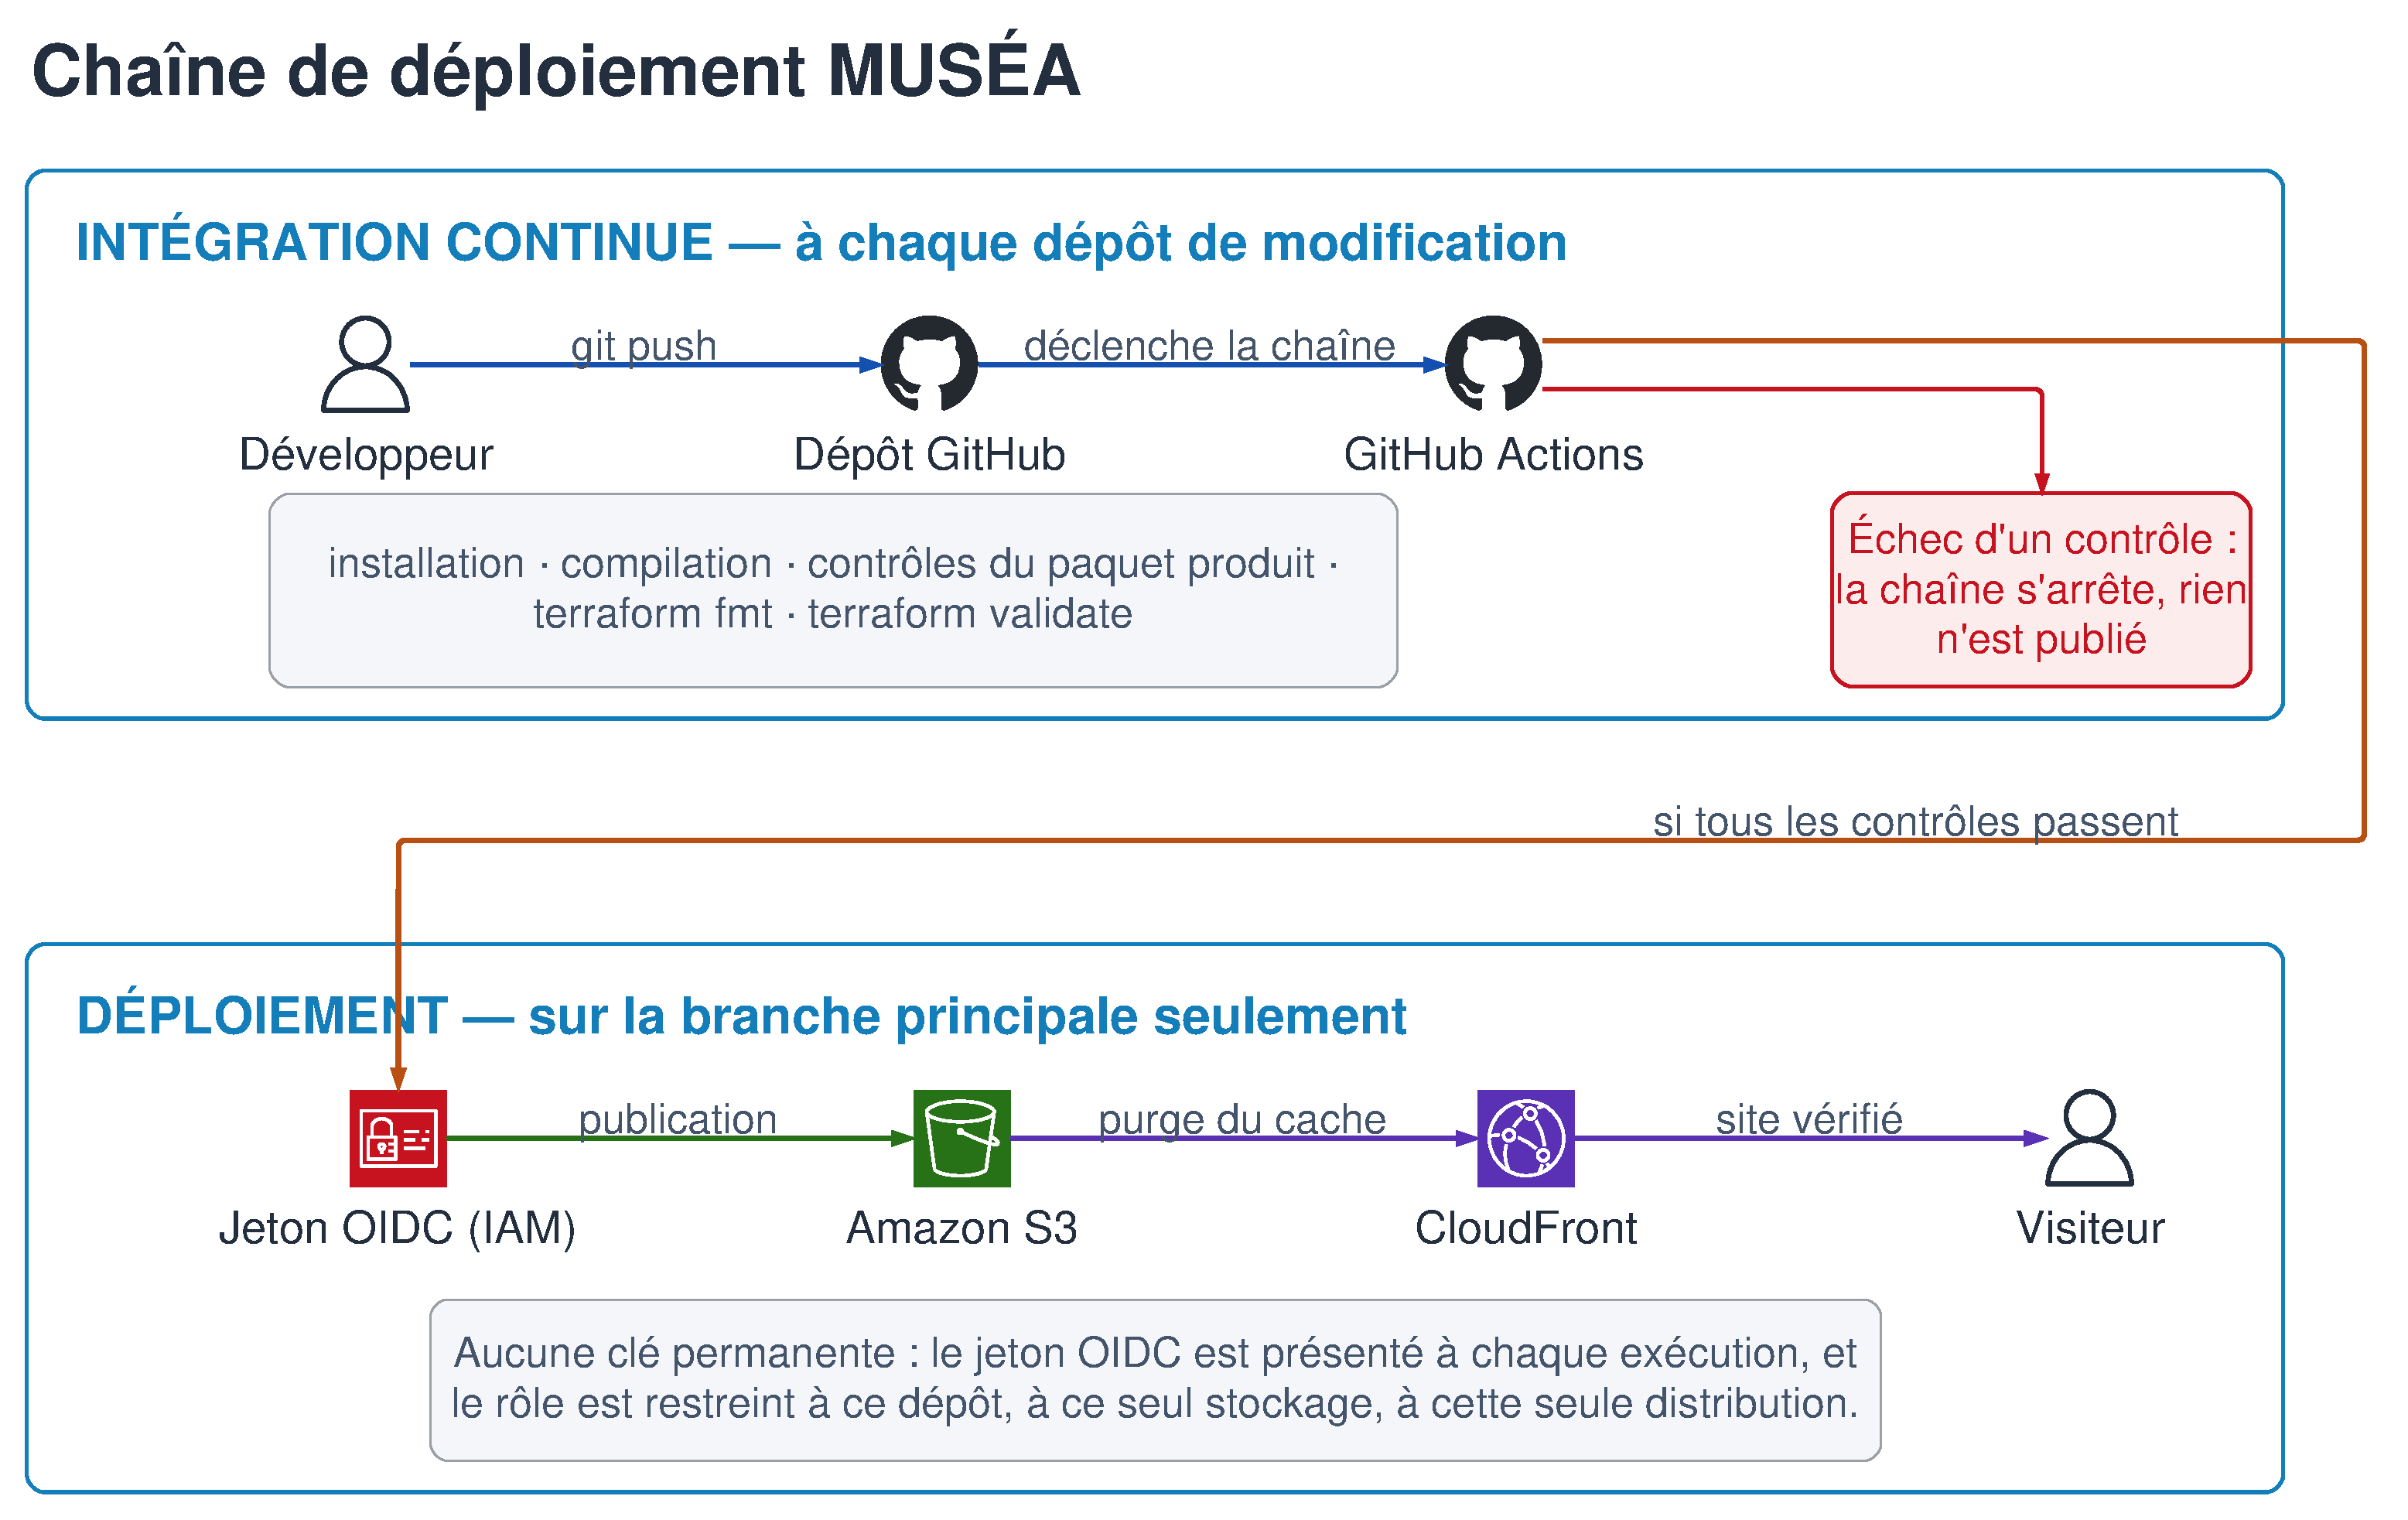
\includegraphics[width=\textwidth]{figures/deploiement-musea.pdf}
\caption{Chaîne d'intégration et de déploiement continus en service}
\label{fig:devops-actuel}
\source{Élaboré par nos soins d'après les fichiers de description des chaînes du projet.}
\end{figure}
% -----------------------------------------------------------------------------
\cleardoublepage
\chapter*{Annexe 16 : Organigramme de la Fondation Jean Félicien Gacha}
\addcontentsline{toc}{chapter}{Annexe 16 : Organigramme de la Fondation Jean Félicien Gacha}

\vspace{0.3cm}

\begin{figure}[htbp]
\centering
\schema{organigramme}
\caption{Organigramme de la Fondation Jean Félicien Gacha}
\label{fig:organigramme}
\source{Élaboré par nos soins à partir des entretiens conduits en juin 2026.}
\end{figure}
% -----------------------------------------------------------------------------
\cleardoublepage
\chapter*{Annexe 17 : Architecture de l'infrastructure d'hébergement en nuage}
\addcontentsline{toc}{chapter}{Annexe 17 : Architecture de l'infrastructure d'hébergement en nuage}

\vspace{0.3cm}

\begin{figure}[htbp]
\centering
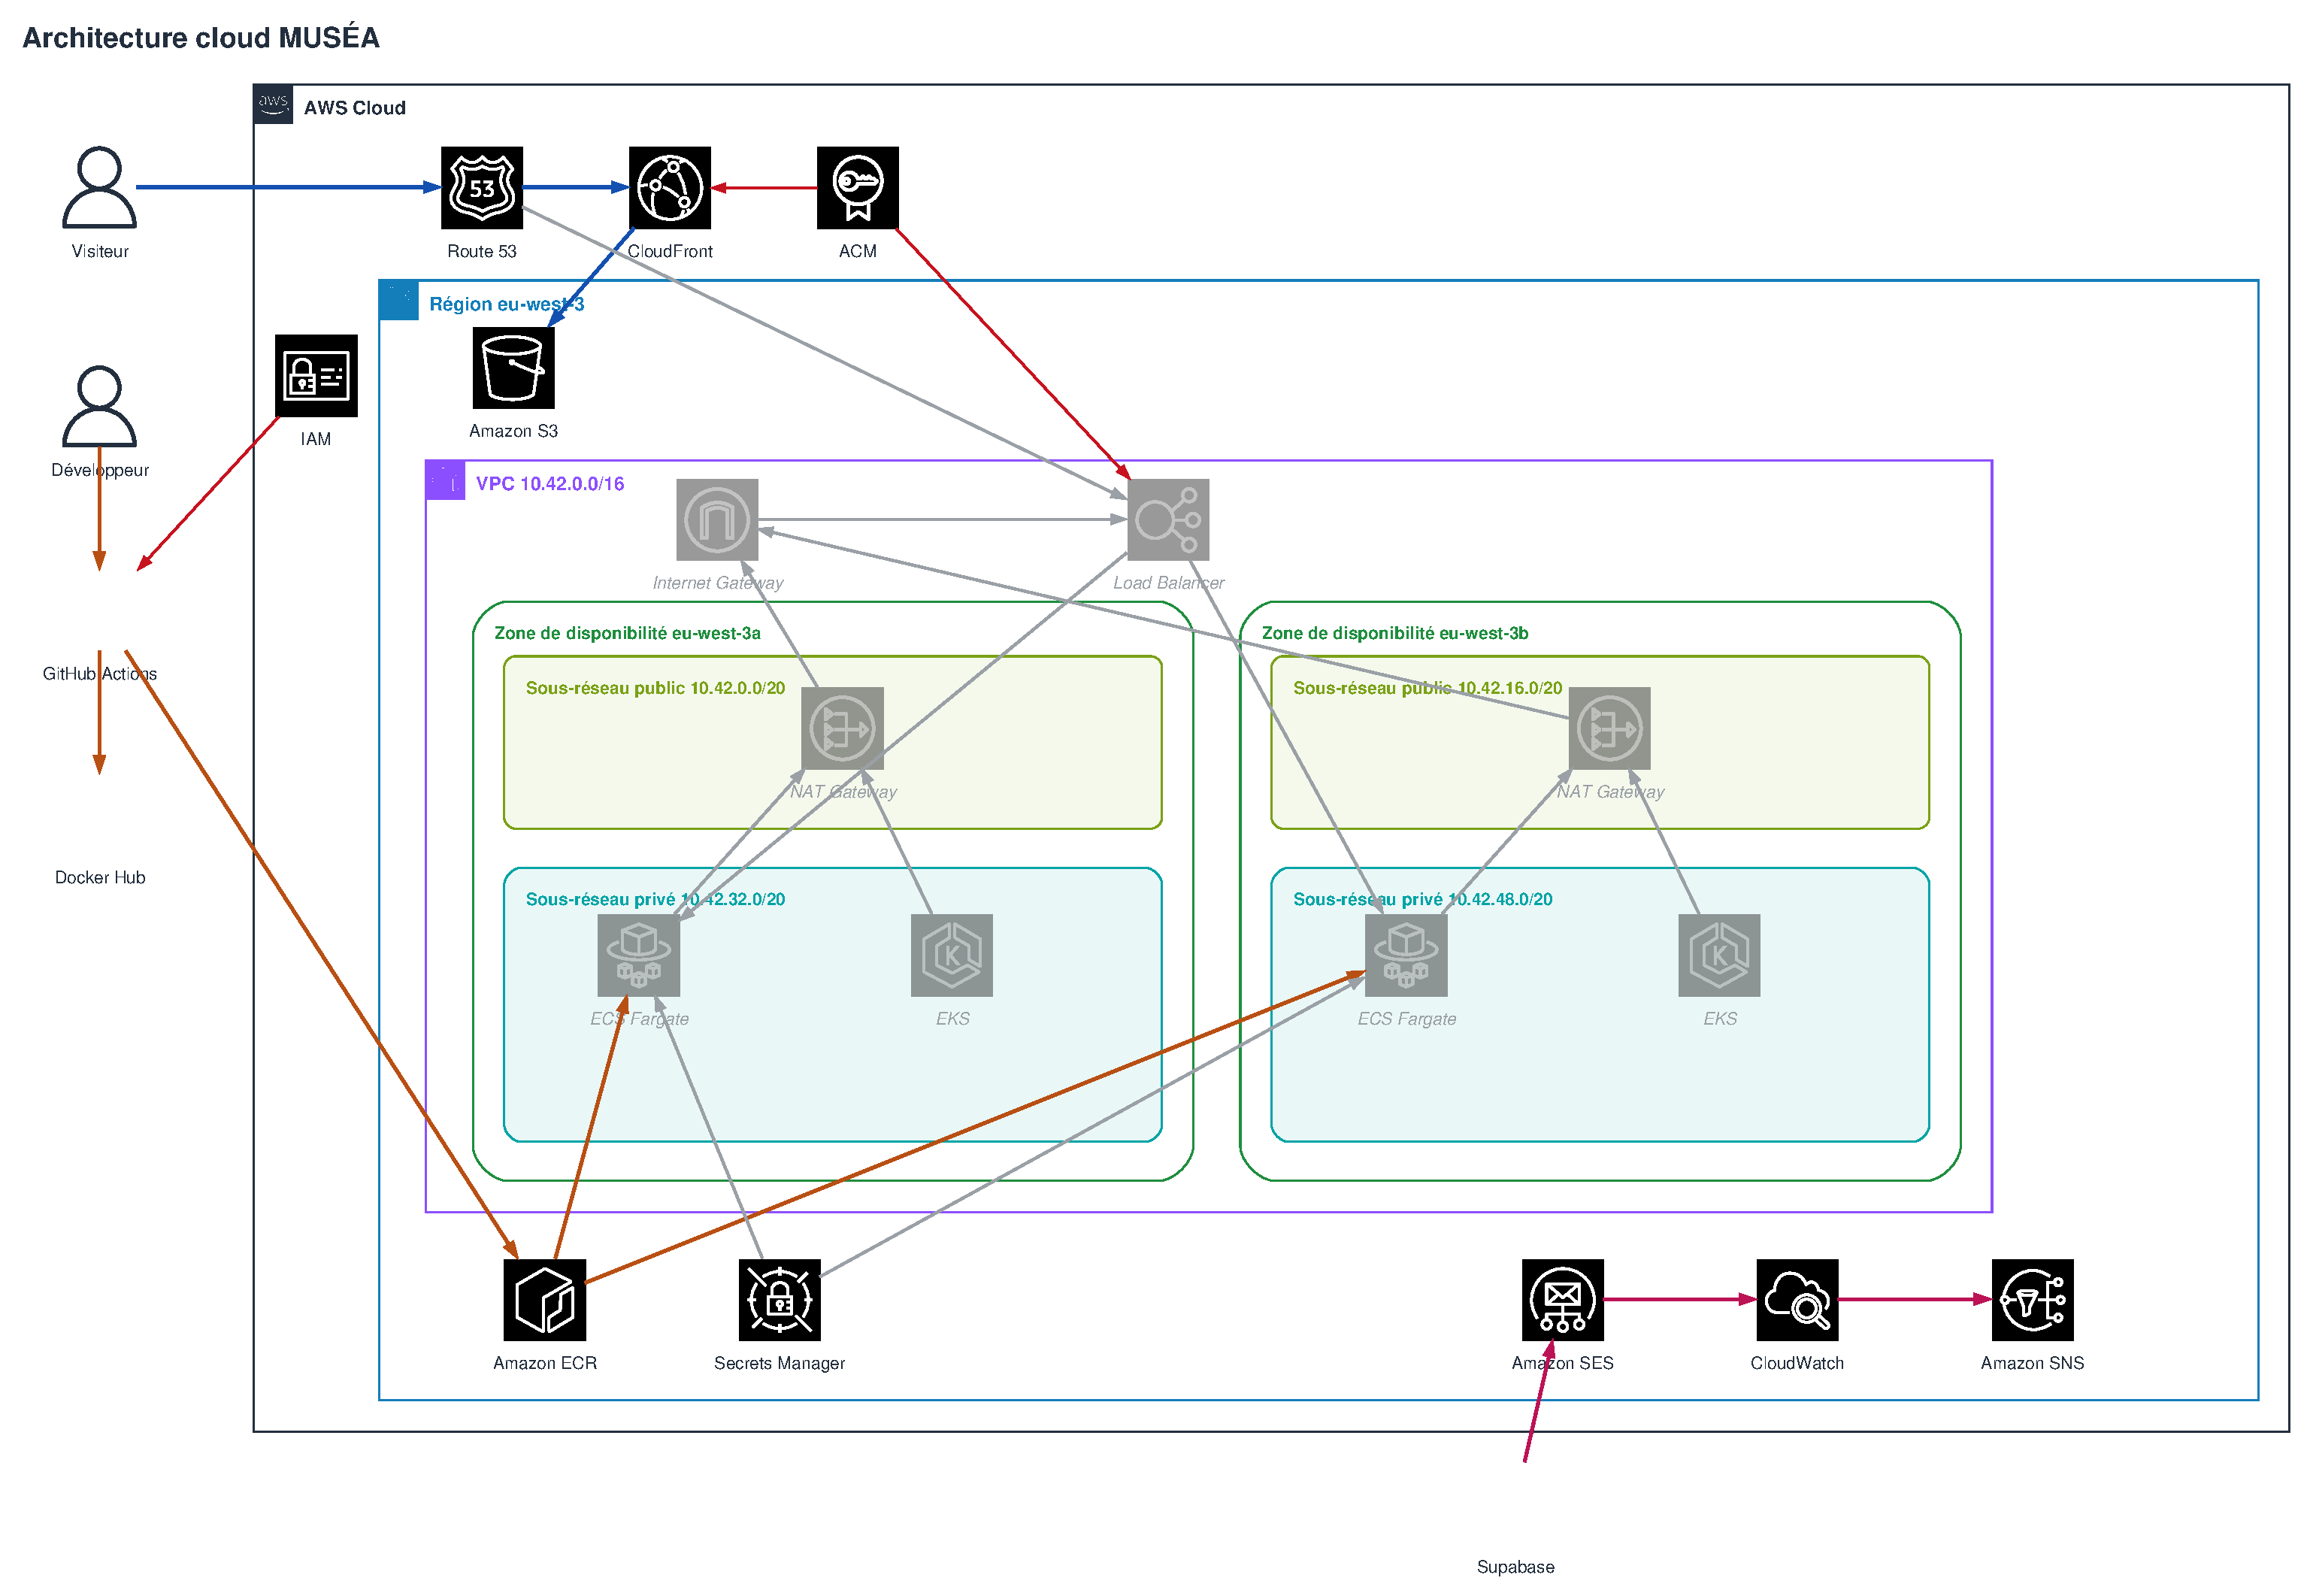
\includegraphics[width=\textwidth]{figures/architecture-cloud-musea.pdf}
\caption{Architecture de l'infrastructure d'hébergement en nuage}
\label{fig:cloud}
\source{Élaboré par nos soins d'après la description Terraform du projet.}
\end{figure}
